% Fig. system overview -- redesigned to separate the PRIMARY paradox test from the
% secondary BOUNDARY checks, with larger fonts (reviewer feedback). TikZ standalone.
\documentclass[border=6pt]{standalone}
\usepackage[T1]{fontenc}
\usepackage{amsmath}
\usepackage{xcolor}
\usepackage{tikz}
\usetikzlibrary{arrows.meta,positioning,calc,fit,backgrounds}

\definecolor{cBB}{HTML}{1B7837}
\definecolor{cGB}{HTML}{9B2226}
\definecolor{cHY}{HTML}{2166AC}
\definecolor{cCT}{HTML}{2B2B2B}
\definecolor{cEV}{HTML}{762A83}
\definecolor{cInk}{HTML}{2B2B2B}
\definecolor{cMut}{HTML}{5A5A5A}

\begin{document}
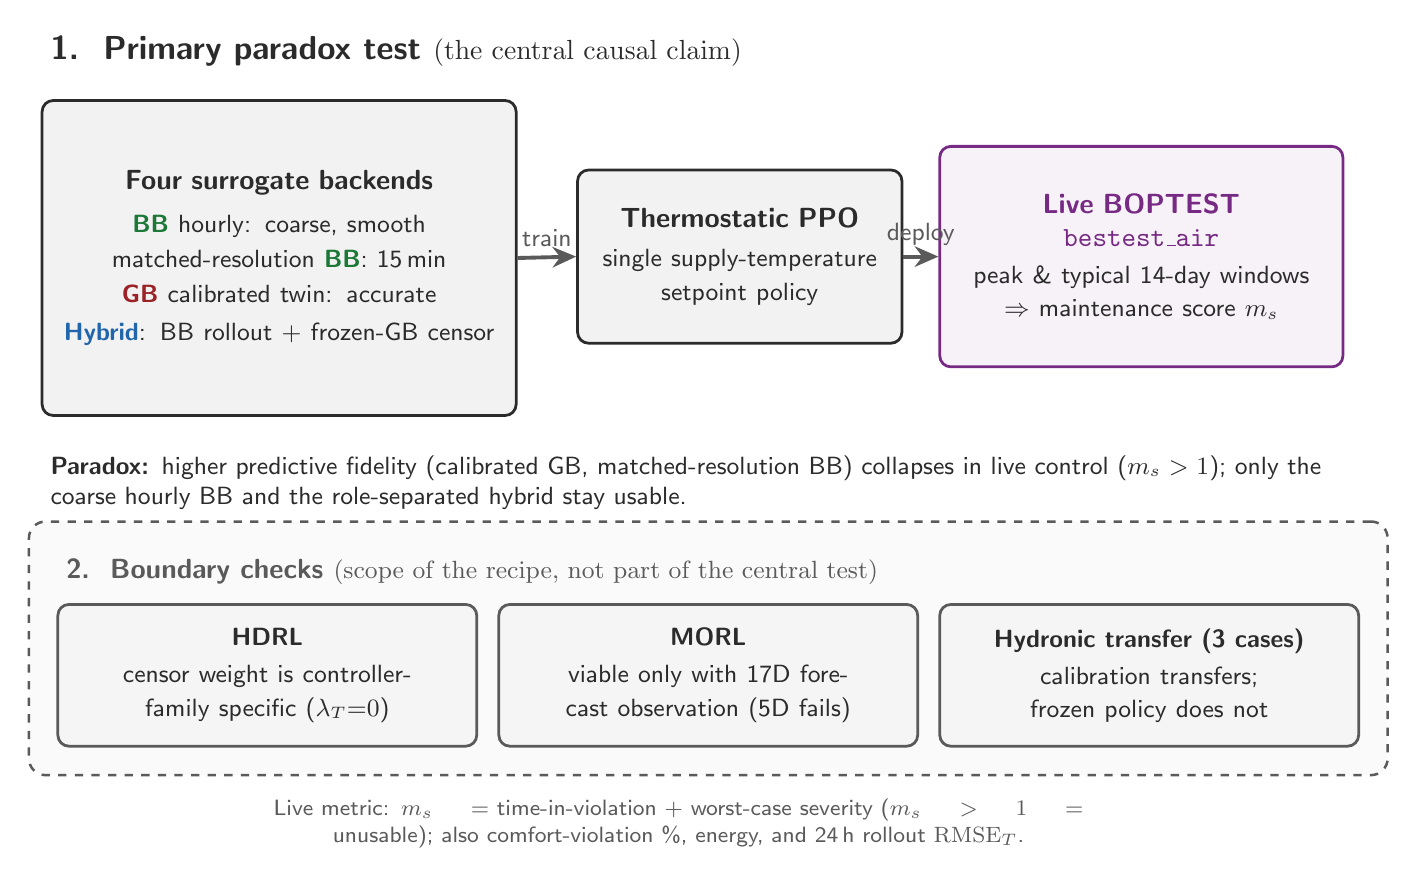
\begin{tikzpicture}[font=\sffamily,
  >={Stealth[length=3mm,width=2.6mm]},
  box/.style={rectangle, rounded corners=4pt, draw=#1, line width=1pt, fill=#1!6,
     align=center, inner sep=2.6mm, text=cInk},
  flow/.style={->, line width=1.4pt, draw=cMut},
  alabel/.style={font=\sffamily\small, text=cMut},
]

% =================== PRIMARY PARADOX TEST ===================
\node[font=\sffamily\bfseries\large, text=cInk, anchor=west] at (0,20mm)
  {1.\ \ Primary paradox test \textnormal{\normalsize(the central causal claim)}};

\node[box=cInk, text width=55mm, minimum height=40mm, anchor=north west] at (0,14mm) (bk)
 {\normalsize\textbf{Four surrogate backends}\\[1.6mm]
  \small
  \textcolor{cBB}{\textbf{BB}} hourly: coarse, smooth\\[0.6mm]
  matched-resolution \textcolor{cBB}{\textbf{BB}}: 15\,min\\[0.6mm]
  \textcolor{cGB}{\textbf{GB}} calibrated twin: accurate\\[0.6mm]
  \textcolor{cHY}{\textbf{Hybrid}}: BB rollout $+$ frozen-GB censor};

\node[box=cCT, text width=36mm, minimum height=22mm, anchor=west] at (68mm,-6mm) (ppo)
 {\normalsize\textbf{Thermostatic PPO}\\[0.8mm]{\small single supply-temperature setpoint policy}};

\node[box=cEV, text width=46mm, minimum height=28mm, anchor=west] at (114mm,-6mm) (live)
 {\normalsize\textbf{\textcolor{cEV}{Live BOPTEST}}\\ \textbf{\textcolor{cEV}{\texttt{bestest\_air}}}\\[0.8mm]
  {\small peak \& typical 14-day windows\\ $\Rightarrow$ maintenance score $m_s$}};

\draw[flow] (bk.east) -- (ppo.west) node[alabel,midway,above]{train};
\draw[flow] (ppo.east) -- (live.west) node[alabel,midway,above]{deploy};

\node[font=\sffamily\small, text=cInk, anchor=north west, text width=162mm] at (0,-30mm)
 {\textbf{Paradox:} higher predictive fidelity (calibrated GB, matched-resolution BB) collapses in live control ($m_s>1$); only the coarse hourly BB and the role-separated hybrid stay usable.};

% =================== BOUNDARY CHECKS ===================
\node[font=\sffamily\bfseries, text=cMut, anchor=west] (btitle) at (2mm,-46mm)
  {2.\ \ Boundary checks \textnormal{\small(scope of the recipe, not part of the central test)}};

\node[box=cMut, text width=48mm, minimum height=18mm, anchor=north west] at (2mm,-50mm) (hd)
 {\small\textbf{HDRL}\\[0.5mm]censor weight is controller-family specific ($\lambda_T{=}0$)};
\node[box=cMut, text width=48mm, minimum height=18mm, anchor=north west] at (58mm,-50mm) (mo)
 {\small\textbf{MORL}\\[0.5mm]viable only with 17D forecast observation (5D fails)};
\node[box=cMut, text width=48mm, minimum height=18mm, anchor=north west] at (114mm,-50mm) (tr)
 {\small\textbf{Hydronic transfer (3 cases)}\\[0.5mm]calibration transfers; frozen policy does not};

\begin{scope}[on background layer]
\node[draw=cMut, dashed, rounded corners=6pt, line width=0.9pt,
      fit=(btitle)(hd)(mo)(tr), inner sep=3.5mm, fill=cMut!3] {};
\end{scope}

% bottom metric note
\node[font=\sffamily\footnotesize, text=cMut, align=center, text width=160mm] at (81mm,-78mm)
 {Live metric: $m_s=$ time-in-violation $+$ worst-case severity ($m_s>1=$ unusable); also comfort-violation \%, energy, and 24\,h rollout $\mathrm{RMSE}_T$.};

\end{tikzpicture}
\end{document}
